\documentclass[0-protokol.tex]{subfiles}
\begin{document}

\subsection*{Úkol 1}
Hodnoty, naměřené přímou metodou měření odporu pomocí zapojení 1$a$, jsou uvedeny v tabulce \ref{tab:u1_a}. Závislost nekorigovaného odporu na proudu je vynesena v grafu \ref{fig:u1_a}, závislost korigovaného odporu na proudu v grafu \ref{fig:u1_a_kor}.
\begin{table}[H] 
\centering
\setlength{\tabcolsep}{10pt}
\begin{tabular}{cccccccc}                                                                                                                   \toprule
$U_a$      & $\sigma_{U_a}$  & $I_a$       & $\sigma_{I_a}$ & $R_a$         & $\sigma_{R_a}$ & $R_{a_{kor}}$ & $\sigma_{R_{a_{kor}}}$   \\
$[\si{V}]$ & $[\si{V}]$      & $[\si{mA}]$ & $[\si{mA}]$    & $[\si{\ohm}]$ & $[\si{\ohm}]$  & $[\si{\ohm}]$ & $[\si{\ohm}]$            \\  \midrule

0.15       & 0.003           & 1.11        &    0.003       & 135.1         & 2.7            & 24.9          & 3.0                      \\                                                                  
0.35       & 0.003           & 4.45        &    0.015       & 78.7          & 0.7            & 38.9          & 1.0                      \\                                                                  
0.51       & 0.003           & 6.30        &    0.015       & 81.0          & 0.5            & 41.2          & 0.9                      \\                                                                  
0.70       & 0.003           & 9.10        &    0.030       & 76.9          & 0.4            & 55.8          & 0.7                      \\                                                                  
0.85       & 0.003           & 10.0        &    0.030       & 85.0          & 0.4            & 63.9          & 0.7                      \\                                                                  
1.09       & 0.003           & 11.0        &    0.030       & 99.1          & 0.4            & 78.0          & 0.7                      \\                                                                  
1.64       & 0.006           & 12.7        &    0.030       & 129.1         & 0.6            & 108.0         & 0.8                      \\                                                                  
2.56       & 0.006           & 15.0        &    0.060       & 170.7         & 0.8            & 159.8         & 0.9                      \\                                                                  
2.90       & 0.006           & 15.8        &    0.060       & 183.5         & 0.8            & 172.6         & 0.9                      \\                                                                  
4.10       & 0.015           & 18.4        &    0.060       & 222.8         & 1.1            & 211.9         & 1.2                      \\                                                                  
5.00       & 0.015           & 20.4        &    0.060       & 245.1         & 1.0            & 234.2         & 1.1                      \\                                                                  
6.25       & 0.015           & 23.4        &    0.060       & 267.1         & 0.9            & 256.2         & 1.1                      \\                                                                  
7.50       & 0.015           & 25.8        &    0.060       & 290.7         & 0.9            & 279.8         & 1.0                      \\                                                                  
8.90       & 0.030           & 28.6        &    0.060       & 311.2         & 1.2            & 300.3         & 1.3                      \\                                                                  
11.4       & 0.030           & 33.0        &    0.150       & 345.5         & 1.8            & 341.4         & 1.8                      \\                                                                  
13.2       & 0.030           & 35.5        &    0.150       & 371.8         & 1.8            & 367.7         & 1.8                      \\                                                                  
15.0       & 0.030           & 38.5        &    0.150       & 389.6         & 1.7            & 385.5         & 1.7                      \\                                                                  
19.1       & 0.060           & 44.0        &    0.150       & 434.1         & 2.0            & 430.0         & 2.0                      \\                                                                  
22.0       & 0.060           & 47.5        &    0.150       & 463.2         & 1.9            & 459.1         & 1.9                      \\  \bottomrule                                                                  

\end{tabular}
\caption{Hodnoty naměřené a vypočtené s použitím zapojení $a$}
\label{tab:u1_a}
\end{table}

\begin{figure}[H] 
\centering
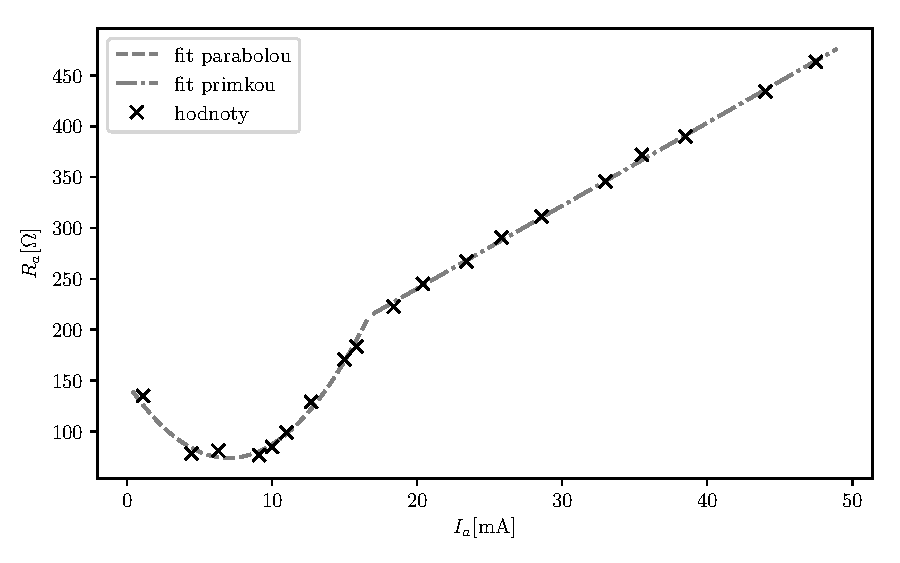
\includegraphics[]{plot/u1_a2}
\caption{Graf závislosti nekorigovaného odporu na proudu pomocí zapojení $a$}
\label{fig:u1_a}
\end{figure}

\begin{figure}[H] 
\centering
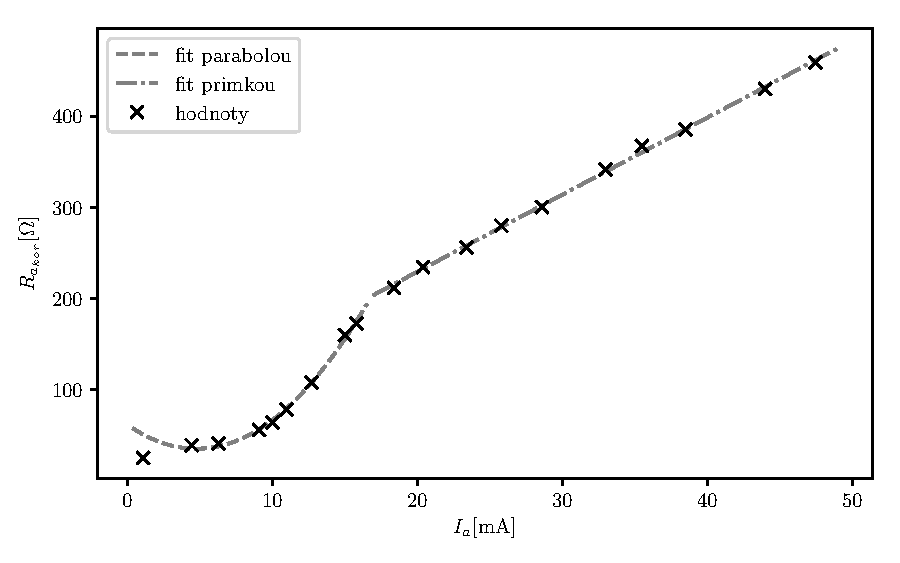
\includegraphics[]{plot/u1_a_kor2}
\caption{Graf závislosti korigovaného odporu na proudu pomocí zapojení $a$}
\label{fig:u1_a_kor}
\end{figure}

Hodnoty, naměřené přímou metodou měření odporu pomocí zapojení 1$b$ jsou uvedeny v tabulce \ref{tab:u1_b}. Závislost nekorigovaného odporu na proudu je vynesena v grafu \ref{fig:u1_b}, závislost korigovaného odporu na proudu v grafu \ref{fig:u1_b_kor}.

\begin{table}[H]
\centering
\setlength{\tabcolsep}{10pt}
\begin{tabular}{cccccccccc}                                                                                                                   \toprule
$U_b$      & $\sigma_{U_b}$  & $I_b$       & $\sigma_{I_b}$ & $I_{b_{kor}}$ & $\sigma_{I_{b_{kor}}}$ & $R_b$         & $\sigma_{R_b}$ & $R_{b_{kor}}$ & $\sigma_{R_{b_{kor}}}$   \\
$[\si{V}]$ & $[\si{V}]$      & $[\si{mA}]$ & $[\si{mA}]$    & $[\si{mA}]$   & $[\si{mA}]$            & $[\si{\ohm}]$ & $[\si{\ohm}]$  & $[\si{\ohm}]$ & $[\si{\ohm}]$            \\  \midrule
                                                                                                                                                                                             
0.15       & 0.003           & 2.41        &    0.006       & 2.60          &    0.01                & 62.2          & 1.3            & 67.7          & 1.5                      \\                                                                  
0.28       & 0.003           & 6.10        &    0.015       & 6.46          &    0.02                & 45.9          & 0.5            & 48.8          & 0.6                      \\                                                                  
0.39       & 0.003           & 7.90        &    0.030       & 8.40          &    0.03                & 49.4          & 0.4            & 52.7          & 0.5                      \\                                                                  
0.50       & 0.003           & 9.40        &    0.030       & 10.0          &    0.03                & 53.2          & 0.4            & 57.1          & 0.4                      \\                                                                  
0.70       & 0.003           & 11.2        &    0.030       & 12.1          &    0.03                & 62.5          & 0.3            & 68.0          & 0.4                      \\                                                                  
0.90       & 0.003           & 12.4        &    0.030       & 13.5          &    0.03                & 72.6          & 0.3            & 80.1          & 0.4                      \\                                                                  
1.10       & 0.003           & 13.4        &    0.030       & 14.8          &    0.03                & 82.1          & 0.3            & 91.9          & 0.4                      \\                                                                  
2.00       & 0.006           & 15.2        &    0.060       & 16.5          &    0.07                & 131.6         & 0.7            & 144.2         & 0.8                      \\                                                                  
3.00       & 0.006           & 18.4        &    0.060       & 20.4          &    0.07                & 163.0         & 0.6            & 182.9         & 0.9                      \\                                                                  
4.00       & 0.015           & 19.8        &    0.060       & 20.8          &    0.06                & 202.0         & 1.0            & 213.5         & 1.1                      \\                                                                  
5.00       & 0.015           & 22.4        &    0.060       & 23.7          &    0.06                & 223.2         & 0.9            & 237.3         & 1.0                      \\                                                                  
6.00       & 0.015           & 25.0        &    0.060       & 26.6          &    0.06                & 240.0         & 0.8            & 256.4         & 1.0                      \\                                                                  
7.20       & 0.015           & 27.6        &    0.060       & 29.5          &    0.07                & 260.9         & 0.8            & 280.4         & 0.9                      \\                                                                  
8.60       & 0.030           & 29.8        &    0.060       & 30.9          &    0.06                & 288.6         & 1.2            & 300.2         & 1.3                      \\                                                                  
13.0       & 0.030           & 37.5        &    0.150       & 39.2          &    0.15                & 346.7         & 1.6            & 363.5         & 1.8                      \\                                                                  
14.8       & 0.030           & 40.5        &    0.150       & 42.4          &    0.15                & 365.4         & 1.5            & 384.2         & 1.7                      \\                                                                  
19.0       & 0.060           & 45.5        &    0.150       & 46.7          &    0.15                & 417.6         & 1.9            & 429.6         & 2.0                      \\                                                                  
21.8       & 0.060           & 49.0        &    0.150       & 50.4          &    0.15                & 444.9         & 1.8            & 458.5         & 1.9                      \\  \bottomrule                                                                  

\end{tabular}

\caption{Hodnoty naměřené a vypočtené s použitím zapojení $b$}
\label{tab:u1_b}
\end{table}

\begin{figure}[H] 
\centering
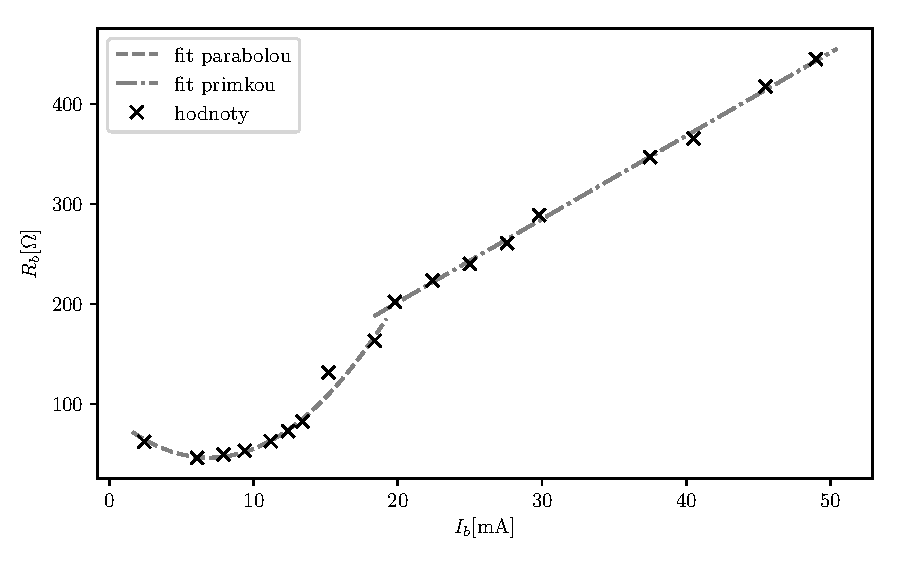
\includegraphics[]{plot/u1_b}
\caption{Graf závislosti nekorigovaného odporu na proudu pomocí zapojení $b$}
\label{fig:u1_b}
\end{figure}

\begin{figure}[H] 
\centering
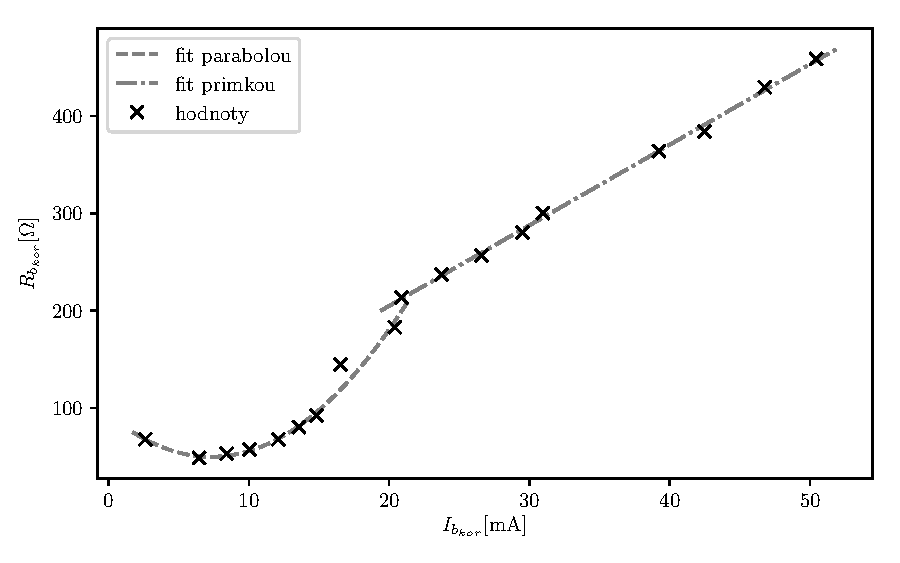
\includegraphics[]{plot/u1_b_kor}
\caption{Graf závislosti korigovaného odporu na proudu pomocí zapojení $b$}
\label{fig:u1_b_kor}
\end{figure}

\subsection*{Úkol 2}
Vnitřní odpor ampérmetru substituční metodou byl měřen pro rozsah $\SI{75}{mA}$. Jako srovnávací proud jsem použil hodnotu $\SI{18 \pm 0,05}{mA}$. Pomocí odporové dekády byla určena hodnota vnitřního odporu ampérmetru $\SI{4,1 \pm 0,004}{\ohm}$.

Vnitřní odpor voltmetru substituční metodou jsem určil pro rozsah $\SI{30}{\volt}$. Použil jsem srovnávací proud  $\SI{1,8 \pm 0,005}{mA}$. Opět pomocí odporové dekády byla určena hodnota vnitřního odporu voltmetru $\SI{15 \pm 0,02}{\kilo\ohm}$.

Odpory zbylých rozsahů jsem měřil digitálním multimetrem. Rozsahu, vhodnému k měření všech hodnot odporů voltmetru, odpovídá chyba $0,8 \percent$  z naměřené hodnoty $\pm 2$ digity, pro hodnoty odporů ampérmetru taktéž $0,8 \percent$ z naměřené hodnoty $\pm 4$ digity. 

\begin{table}[H]
\parbox{.45\linewidth}{ \label{tab:odpory_A}
\centering
\setlength{\tabcolsep}{15pt}
\begin{tabular}{ccc}                                        \toprule
rozsah      &  odpor           &   chyba                   \\  
$[\si{mA}]$ &  $[\si{\ohm}]$   &   $[\si{\ohm}]$           \\  \midrule
1,5         &  110,2           &   1,3                     \\
3           &  82,9            &   1,1                     \\
7,5         &  39,8            &   0,7                     \\
15          &  21,1            &   0,6                     \\
30          &  10,9            &   0,5                     \\
75          &  4,5             &   0,4                     \\  \bottomrule
\end{tabular}
\caption{Odpory ampérmetru měřené digitálním multimetrem}
\label{tab:ampermetr}
}
\hfill
\parbox{.45\linewidth}{ \label{tab:odpory_V}
\centering
\setlength{\tabcolsep}{15pt}
\begin{tabular}{ccc}                                           \toprule
rozsah      &  odpor           &   chyba                   \\  
$[\si{V}]$  &  $[\si{\ohm}]$   &   $[\si{\ohm}]$           \\  \midrule
1,5         &    770           &   8                       \\
3           &   1500           &   32                      \\
7,5         &   3750           &   50                      \\
15          &   7480           &   80                      \\
30          &  14970           &   140                     \\  \bottomrule
\end{tabular}





\caption{Odpory voltmetru měřené digitálním multimetrem}
\label{tab:voltmetr}
}
\end{table}

\newpage

\subsection*{Úkol 3}

Následující tabulka obsahuje hodnoty proudu a odporu měřené substituční metodou.

\begin{table}[H] 
\centering
\setlength{\tabcolsep}{10pt}
\begin{tabular}{SSSS}                                              \\ \toprule
{$I$}         & {$\sigma_I$}   & {$R$}           & {$\sigma_R$}    \\
{$[\si{mA}]$} & {$[\si{mA}]$}  & {$[\si{\ohm}]$} & {$[\si{\ohm}]$} \\ \midrule
0.9800        & 0.0030         &  42.40          & 0.04            \\
 1.980        & 0.006          &  42.40          & 0.04            \\
 2.800        & 0.006          &  43.40          & 0.04            \\
 4.100        & 0.015          &  45.00          & 0.04            \\
 4.950        & 0.015          &  46.20          & 0.05            \\
 6.900        & 0.015          &  50.10          & 0.05            \\
 9.100        & 0.030          &  59.00          & 0.06            \\
10.900        & 0.030          &  76.00          & 0.08            \\
13.100        & 0.030          & 121.00          & 0.12            \\
15.000        & 0.030          & 158.00          & 0.16            \\
20.00         & 0.06           & 230.00          & 0.23            \\
25.00         & 0.06           & 275.00          & 0.28            \\
30.00         & 0.06           & 317.00          & 0.32            \\
35.00         & 0.15           &  361.0          & 0.4             \\
40.00         & 0.15           &  403.0          & 0.4             \\
45.00         & 0.15           &  437.0          & 0.4             \\
50.00         & 0.15           &  473.0          & 0.5             \\ \bottomrule
\end{tabular}

\caption{Závislost odporu na proudu měřená substituční metodou}
\label{tab:u3}
\end{table}

\newpage

V grafu \ref{fig:u3} je znázorněna závislost odporu vlákna žárovky na procházejícím proudu. Data jsou opět proložena kvadratickým a lineárním fitem.
\begin{figure}[H]
\centering
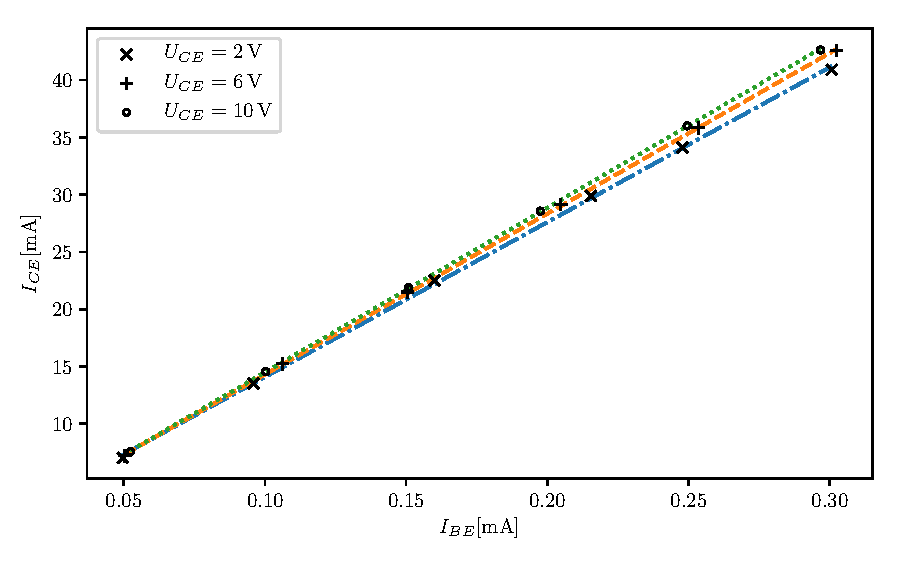
\includegraphics[]{u3}
\caption{Graf závislosti odporu na proudu měřené substituční metodou}
\label{fig:u3}
\end{figure}

Odpor byl změřen také digitálním multimetrem, výsledkem je hodnota $R = \SI{43.0 \pm 0.3}{\ohm}.$

\newpage

\subsection*{Úkol 5}
Závislost podle rovnice \eqref{eq:regrese} je vyobrazena v grafu \ref{fig:u5}. Bylo použito prvních 6 hodnot z úkolu 3. Pomocí lineární regrese byla určena hodnota odporu žárovky při pokojové teplotě $\SI{42.35 \pm 0.09}{\ohm}$.

\begin{figure}[H]
\centering
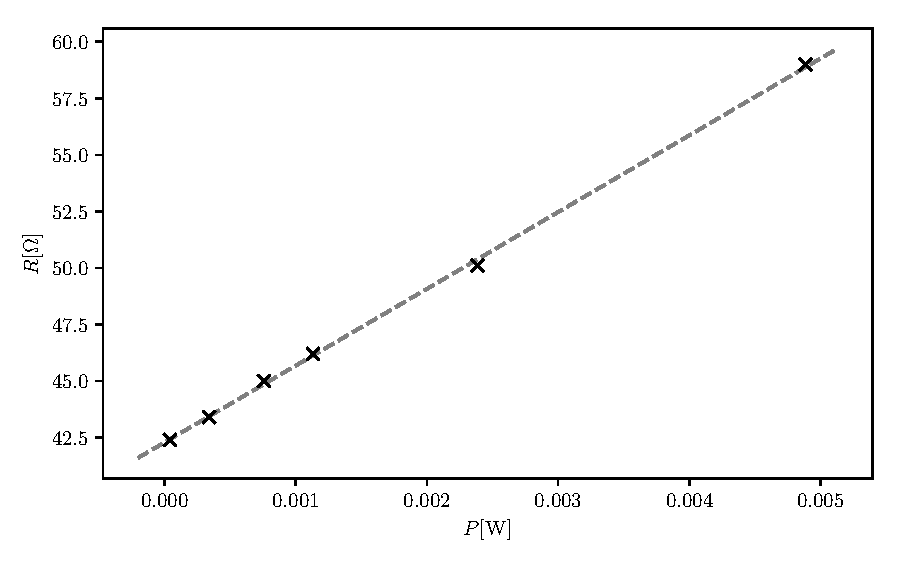
\includegraphics[]{u5}
\caption{Lineární závislost prvních šesti hodnot příkonu a odporu}
\label{fig:u5}
\end{figure}

\end{document}
